% Native tensor-operation graph. Compile with pdflatex.
% The first arrow includes the local trace-difference estimate and
% extension of a nonnegative restricted sum to the full index range.
\documentclass[tikz,border=11pt]{standalone}
\usepackage[T1]{fontenc}
\usepackage{lmodern,amsmath,amssymb}
\usetikzlibrary{arrows.meta,calc}
\definecolor{ink}{HTML}{183444}
\definecolor{blue}{HTML}{1B6780}
\definecolor{amber}{HTML}{AD601A}
\definecolor{pale}{HTML}{F2F6F8}
\begin{document}
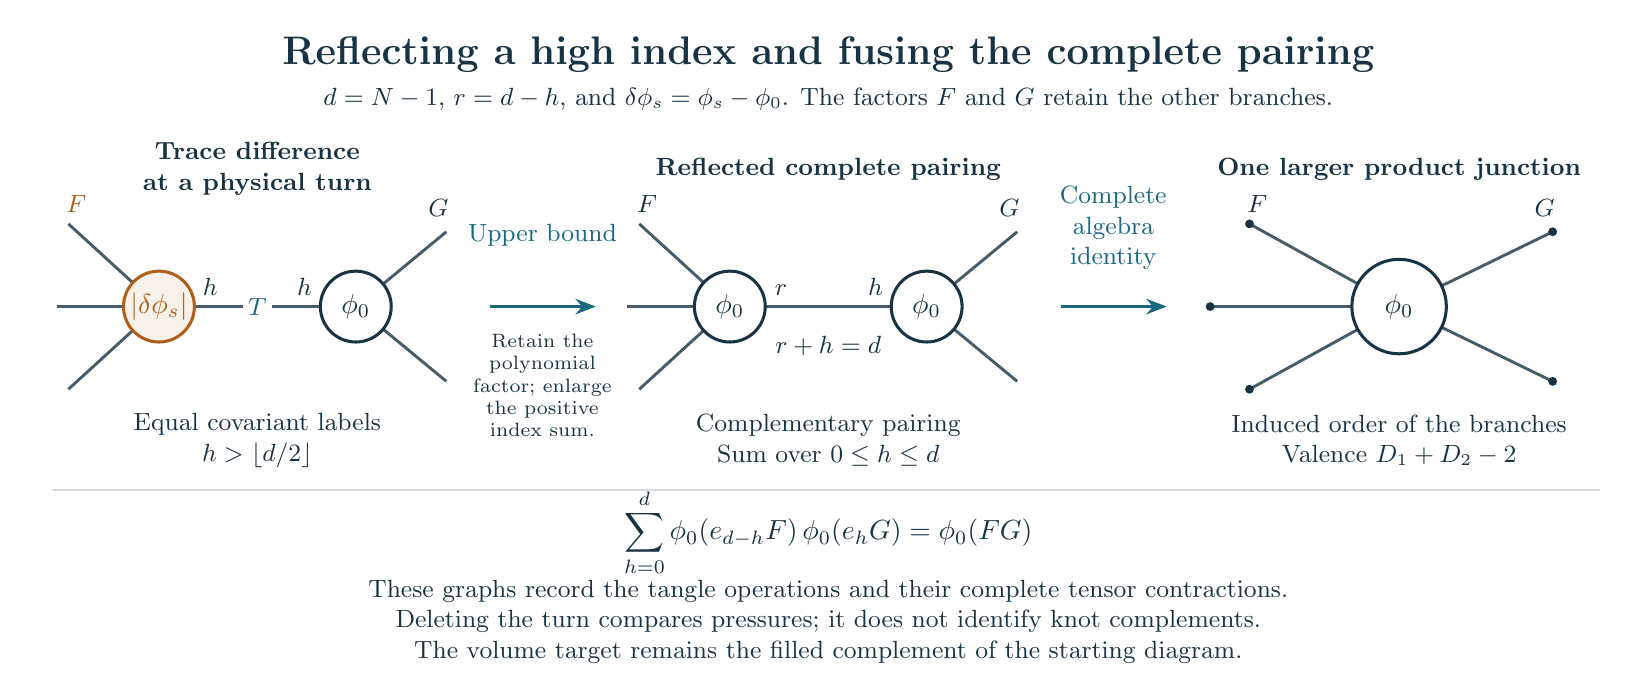
\begin{tikzpicture}[x=1cm,y=1cm,font=\sffamily,text=ink,
  line width=1.05pt,
  vertex/.style={circle,draw=ink,fill=white,minimum size=9mm,
    inner sep=1pt,line width=1.1pt,font=\normalsize},
  difference/.style={vertex,draw=amber,fill=amber!9,text=amber},
  edge/.style={draw=ink!80,line width=1.05pt},
  comparison/.style={-{Stealth[length=2.6mm]},draw=blue,line width=1.25pt}]

\node[font=\Large\bfseries] at (9.8,7.15)
  {Reflecting a high index and fusing the complete pairing};
\node[font=\small,align=center] at (9.8,6.58)
  {$d=N-1$, $r=d-h$, and $\delta\phi_s=\phi_s-\phi_0$.
   The factors $F$ and $G$ retain the other branches.};

\node[font=\small\bfseries,align=center,text width=5.6cm] at (2.55,5.7)
  {Trace difference at a physical turn};
\node[font=\small\bfseries,align=center,text width=5.7cm] at (9.8,5.7)
  {Reflected complete pairing};
\node[font=\small\bfseries,align=center,text width=5.2cm] at (17.05,5.7)
  {One larger product junction};

% First panel: valences four and three; all other branches are retained.
\coordinate (a) at (1.3,3.95);
\coordinate (b) at (3.8,3.95);
\draw[edge] (.15,5.0)--(a)--(.15,2.9);
\draw[edge] (.0,3.95)--(a);
\draw[edge] (b)--(4.95,4.9);
\draw[edge] (b)--(4.95,3.0);
\draw[edge] (a)--(b);
\node[difference] at (a) {$\lvert\delta\phi_s\rvert$};
\node[vertex] at (b) {$\phi_0$};
\node[font=\small,above] at (1.95,3.95) {$h$};
\node[font=\small,above] at (3.15,3.95) {$h$};
\node[fill=white,inner sep=2pt,font=\small,text=blue] at (2.55,3.95) {$T$};
\node[font=\small,align=center] at (2.55,2.25)
  {Equal covariant labels\\$h>\lfloor d/2\rfloor$};
\node[font=\small,text=amber] at (.25,5.25) {$F$};
\node[font=\small] at (4.85,5.2) {$G$};

% First comparison is an inequality, including positive enlargement.
\draw[comparison] (5.5,3.95)--(6.85,3.95);
\node[font=\small,align=center,text width=2.1cm,text=blue] at (6.17,4.85)
  {Upper bound};
\node[font=\scriptsize,align=center,text width=2.2cm] at (6.17,2.95)
  {Retain the polynomial factor; enlarge the positive index sum.};

% Second panel: one index was reflected; the full sum is complementary.
\coordinate (c) at (8.55,3.95);
\coordinate (e) at (11.05,3.95);
\draw[edge] (7.4,5.0)--(c)--(7.4,2.9);
\draw[edge] (7.25,3.95)--(c);
\draw[edge] (e)--(12.2,4.9);
\draw[edge] (e)--(12.2,3.0);
\draw[edge] (c)--(e);
\node[vertex] at (c) {$\phi_0$};
\node[vertex] at (e) {$\phi_0$};
\node[font=\small,above] at (9.2,3.95) {$r$};
\node[font=\small,above] at (10.4,3.95) {$h$};
\node[font=\small] at (9.8,3.45) {$r+h=d$};
\node[font=\small,align=center] at (9.8,2.25)
  {Complementary pairing\\Sum over $0\le h\le d$};
\node[font=\small] at (7.5,5.25) {$F$};
\node[font=\small] at (12.1,5.2) {$G$};

% Second comparison is the exact complete Frobenius identity.
\draw[comparison] (12.75,3.95)--(14.1,3.95);
\node[font=\small,align=center,text width=2.2cm,text=blue] at (13.42,4.95)
  {Complete algebra\\identity};

% The induced boundary order is unchanged after contracting the band.
\coordinate (f) at (17.05,3.95);
\draw[edge] (15.15,5.0)--(f)--(15.15,2.9);
\draw[edge] (14.65,3.95)--(f);
\draw[edge] (f)--(19.0,4.9);
\draw[edge] (f)--(19.0,3.0);
\node[vertex,minimum size=12mm] at (f) {$\phi_0$};
\foreach \p in {(15.15,5.0),(14.65,3.95),(15.15,2.9),(19.0,4.9),(19.0,3.0)}
  \fill[ink] \p circle[radius=1.6pt];
\node[font=\small,align=center] at (17.05,2.25)
  {Induced order of the branches\\Valence $D_1+D_2-2$};
\node[font=\small] at (15.25,5.25) {$F$};
\node[font=\small] at (18.9,5.2) {$G$};

\draw[ink!18] (-.05,1.62)--(19.6,1.62);
\node[font=\normalsize] at (9.8,1.08)
  {$\displaystyle
    \sum_{h=0}^{d}\phi_0(e_{d-h}F)\,\phi_0(e_hG)=\phi_0(FG)$};
\node[font=\small,align=center,text width=19.3cm] at (9.8,-.05)
  {These graphs record the tangle operations and their complete tensor contractions.\\
   Deleting the turn compares pressures; it does not identify knot complements.\\
   The volume target remains the filled complement of the starting diagram.};
\end{tikzpicture}
\end{document}
